\documentclass[12pt]{article}

\usepackage{fancyhdr}
\usepackage{amsmath}
\usepackage{amssymb}
\usepackage{graphicx}
\usepackage[a4paper,twoside,left=3.0cm,right=3.0cm,top=3.5cm,bottom=3.0cm]{geometry}
\usepackage{url}
\usepackage{hyperref}

\hypersetup{pdfauthor={Pedro Brandimarte},
  pdftitle={SatisfyMe},
  pdfsubject={k-SAT problem},
  pdfkeywords={k-SAT CNF Knuth dancing links X},
  pdfproducer={Latex with hyperref},
  pdfcreator={pdflatex}
}

\linespread{1.5}

\setlength{\unitlength}{1mm}
\setlength{\headheight}{15pt}

\pagestyle{fancy}
\renewcommand{\sectionmark}[1]{\markright{\thesection\ #1}}
\fancyhead{}
\fancyfoot{}
\fancyhead[LE,RO]{\bfseries\thepage}
\fancyhead[LO,RE]{\nouppercase{\emph{\bfseries\rightmark}}}
\fancyfoot[CO,CE]{\bfseries SatisfyMe!}
\renewcommand{\headrulewidth}{0.5pt}
\renewcommand{\footrulewidth}{0.5pt}


%---------------------------------------------------------------------
\begin{document}

\thispagestyle{empty}

\title{SatisfyMe!\\[10pt]}

\author{Pedro Brandimarte\\[20pt]}

\date{\small{\today}}

\maketitle

%---------------------------------------------------------------------
\vspace{50pt}
\section{Objective}

Given a set $U = \left\{ x_{_1} , \, x_{_2} , \dots , \, x_n \right\}$ of boolean variables (literals) and a boolean formula $k$-CNF (conjunctive normal form composed by ``and'' of clauses in $\left\{ c_{_1} , \, c_{_2} , \dots , \, c_m \right\}$, where each clause consists in ``or'' of $k$ literals belonging to the set $U$ plus respective negations), the main objective of this program consists on searching attributions (true and false) for the set of literals such that the $k$-CNF is satisfied (true).
This is a NP-complete problem known as $k$-SAT.

The $k$-SAT problem can be interpreted as a generalized cover set problem and, therefore, can be solved by a backtracking algorithm based on the D. Knuth's ``Dancing Links X'' algorithm~\cite{knuthDLX}.

Besides solving the $k$-SAT problem, the code is also able to determine the solutions, if any, of an exact cover set problem.

\newpage


%---------------------------------------------------------------------

\section{Input and Output}

For the $k$-CNF, the program reads an input from \texttt{stdin} containing integer numbers, where the first line corresponds to ``$k$ $n$ $m$'' (amount of literals, cardinal of $U$ and number of clauses, respectively) and the following lines correspond to the clauses, where a number $i$ represents the variable $x_i$ and $- i$ its negation $\lnot x_i$.

The program output is send to \texttt{stdout}.
With the command line option \texttt{-n} the code prints out the number of different attributions that satisfy the input.
With the option \texttt{-N}, besides printing the number of attributions that satisfy the input, the code also prints all these attributions, line by line and in lexicographical order.
In case no option is passed through the command line, the code prints 1 if the $k$-CNF is satisfiable or 0, otherwise.

The command line option \texttt{-C} indicates that the input contains an exact cover set problem.
In this case, the input represents the problem of covering a set $[n] = \left\{ 1 , \, 2 , \dots , \, n \right\}$ with elements from a collection of $m$ subsets of $[n]$.
The first line corresponds to ``$n$ $m$'' (indicating the set $[n]$ and the amount of subsets of $[n]$, respectively) and the following $m$ lines correspond to the subsets of $[n]$, represented by integers belonging to $[n]$ in ascending order.
As output, the code prints out the number of different solutions for the problem, followed by the respectively solutions, line by line and represented by numbers belonging to $[n]$ in ascending order.


%---------------------------------------------------------------------

\section{\emph{k}-SAT as a Cover Set Problem}
\label{sec:ksatcover}

The $k$-SAT problem can be interpreted as a generalized cover set problem.
Adopting the convention ``1 = true'' and ``0 = false'', one can represent a $k$-SAT by a matrix with the rows containing the possible values for which the variables $\left\{ x_{_1} , \, x_{_2} , \dots , \, x_n \right\}$ can assume (0 or 1), and with the primary columns corresponding to the literals (columns that should be exactly covered, i.e., the subset of rows from a solution must contain exactly one ``1'' at each of those columns) and the secondary columns corresponding to the clauses $\left\{ c_{_1} , \, c_{_2} , \dots , \, c_m \right\}$ which should be covered at least once by the set of rows of a given solution.

For example, consider the input:

\begin{displaymath}
  \begin{array}{c c c}
    3 & 4 & 5 \\
    -1 & 2 & 3 \\
    1 & -2 & 4 \\
    1 & -3 & 4 \\
    -1 & -2 & 3 \\
    -1 & 2 & -3
  \end{array}
\end{displaymath}
\\
which corresponds to the following $k$-CNF:
\begin{displaymath}
  ( \lnot x_{_1} \lor x_{_2} \lor x_{_3} ) \land ( x_{_1} \lor \lnot x_{_2} \lor x_{_4} ) \land ( x_{_1} \lor \lnot x_{_3} \lor x_{_4} ) \land ( \lnot x_{_1} \lor \lnot x_{_2} \lor x_{_3} ) \land ( \lnot x_{_1} \lor x_{_2} \lor \lnot x_{_3} )
\end{displaymath}
\\[-25pt]

Therefore, this boolean formula can be represented by the matrix:

\begin{gather*}
  \begin{matrix}
    \qquad \;\;\;\, \mathrm{x_{_1}} & \, \mathrm{x_{_2}} & \, \mathrm{x_{_3}} & \, \mathrm{x_{_4}} & \, \mathrm{c_{_1}} & \, \mathrm{c_{_2}} & \, \mathrm{c_{_3}} & \, \mathrm{c_{_4}} & \, \mathrm{c_{_5}}
  \end{matrix} \\
  \begin{matrix}
    \mathrm{x_{_1} = 0} \\
    \mathrm{x_{_1} = 1} \\
    \mathrm{x_{_2} = 0} \\
    \mathrm{x_{_2} = 1} \\
    \mathrm{x_{_3} = 0} \\
    \mathrm{x_{_3} = 1} \\
    \mathrm{x_{_4} = 0} \\
    \mathrm{x_{_4} = 1}
  \end{matrix}
  \begin{bmatrix}
    \;1\; & \;0\; & \;0\; & \;0\; & \;1\; & \;0\; & \;0\; & \;1\; & \;1\; \\
    \;1\; & \;0\; & \;0\; & \;0\; & \;0\; & \;1\; & \;1\; & \;0\; & \;0\; \\
    \;0\; & \;1\; & \;0\; & \;0\; & \;0\; & \;1\; & \;0\; & \;1\; & \;0\; \\
    \;0\; & \;1\; & \;0\; & \;0\; & \;1\; & \;0\; & \;0\; & \;0\; & \;1\; \\
    \;0\; & \;0\; & \;1\; & \;0\; & \;0\; & \;0\; & \;1\; & \;0\; & \;1\; \\
    \;0\; & \;0\; & \;1\; & \;0\; & \;1\; & \;0\; & \;0\; & \;1\; & \;0\; \\
    \;0\; & \;0\; & \;0\; & \;1\; & \;0\; & \;0\; & \;0\; & \;0\; & \;0\; \\
    \;0\; & \;0\; & \;0\; & \;1\; & \;0\; & \;1\; & \;1\; & \;0\; & \;0\;
  \end{bmatrix}
\end{gather*}
\\

Thus, as the primary columns (first four) correspond to an exact cover set problem, once selected the row $\mathrm{x_{_i} = 0}$, the row $\mathrm{x_{_i} = 1}$ cannot be in the solution, and vice-versa.
However, the same criteria cannot be used for the columns representing the clauses, since a clause is satisfied when one or more literals are true.

In the example above, one attribution that satisfies the $k$-CNF is $x_{_1}$, $x_{_2}$ and $x_{_3}$ true and $x_{_4}$ false, represented by the rows $x_{_1} = 1$, $x_{_2} = 1$, $x_{_3} = 1$ and $x_{_4} = 0$ (or, in a compact form, 1110).


%---------------------------------------------------------------------

\section{The X Algorithm}
\label{sec:algX}

The X algorithm from D. Knuth \cite{knuthDLX} is a backtracking search algorithm that can be applied to a class of combinatorial puzzle problems, that is to find all solutions of an exact cover problem.
It's based on a technique called \emph{dancing links}: given a pointer $x$ to an element from a double linked list, and let $L{\left[ x \right]}$ and $R{\left[ x \right]}$ be the pointers to the precedent and posterior elements, respectively, then the removal of $x$ from the list is given by the operations:
\\[-5pt]
\begin{displaymath}
  \begin{array}{c c c}
    L{\left[ R{\left[ x \right]} \right]} & \longleftarrow & L{\left[ x \right]} \\
    R{\left[ L{\left[ x \right]} \right]} & \longleftarrow & R{\left[ x \right]}
  \end{array}
\end{displaymath}
\\[-25pt]

However, since after removal the element pointed by $x$ is still allocated in memory, its return to the list is given by the operations:

\begin{displaymath}
  \begin{array}{c c c}
    L{\left[ R{\left[ x \right]} \right]} & \longleftarrow & x \quad \\
    R{\left[ L{\left[ x \right]} \right]} & \longleftarrow & x \quad
  \end{array}
\end{displaymath}
\\
what allow thus return back to the previous stage (\emph{backtrack}).

Given a matrix $A$ of ``0s'' and ``1s'', the X algorithm searches for all sets of rows containing exactly one ``1'' at each column.
The matrix $A$ is then represented only by the ``1s'', with circular double linked lists for the rows and columns.

Each ``1'' in the matrix is represented by an structure containing four pointers for the preceding and posterior elements in the row and column, in addition to a pointer to the head of the column which it belongs to:
\\[-5pt]

\linespread{0.8}

{\footnotesize
  \begin{quote}
\begin{verbatim}
typedef struct node_struct {
   struct node_struct *left, *right; /* predecessor and successor at row */
   struct node_struct *up, *down; /* predecessor and successor at column */
   struct col_struct *col; /* column containing this node */
} node;
\end{verbatim}
  \end{quote}
}

\linespread{1.5}

The columns' lists possess a head and the heads themselves also form a circular double linked list with a head called ``root''.
Each element from a column list has an identifier given by a \emph{string}, a counter with the updated amount of elements in the column and pointers to the precedent and posterior elements in the list and to the root:
\\[-5pt]

\linespread{0.8}

{\footnotesize
  \begin{quote}
\begin{verbatim}
typedef struct col_struct {
   node head; /* list head (root) */
   int len; /* actual number of items in this column list (not including head) */
   char name[max_name]; /* symbolic identifier of the column for printing */
   struct col_struct *prev, *next; /* neighbor columns */
} column;
\end{verbatim}
  \end{quote}
}

\linespread{1.5}

The X algorithm scans the matrix $A$ searching recursively for solutions as follows:
\\[-10pt]

\linespread{0.8}

{\small
  \begin{quote}
    \texttt{If $A$ is empty, print actual solution and return.}

    \texttt{Otherwise, choose a column $c$ and do:}

       \hspace{0.5cm}\texttt{Cover column $c$.}

       \hspace{0.5cm}\texttt{For $r \leftarrow D{\left[ c \right]} , \, D{\left[ D{\left[ c \right]} \right]} , \dots$, while $r \neq c$, do:}

          \hspace{1cm}\texttt{Include $r$ in the partial solution: $partial \leftarrow r$}

          \hspace{1cm}\texttt{For $j \leftarrow R{\left[ r \right]}, \, R{\left[ R{\left[ r \right]} \right]} , \dots$, while $j \neq r$, do:}

             \hspace{1.5cm}\texttt{Cover column from $j$ (i.e.\ $C \left[ j \right]$).}

          \hspace{1cm}\texttt{Recursively call this algorithm for the reduced matrix $A$.}

          \hspace{1cm}\texttt{Assign previous values: $r \leftarrow partial$ and $c \leftarrow c[r]$}

          \hspace{1cm}\texttt{For $j \leftarrow L{\left[ r \right]}, \, L{\left[ L{\left[ r \right]} \right]} , \dots$, while $j \neq r$, do:}

             \hspace{1.5cm}\texttt{Uncover column $C \left[ j \right]$.}

    \texttt{Uncover column $c$.}
  \end{quote}
}

\linespread{1.5}

\noindent where $D$, $U$, $L$ and $R$ are pointers to the elements above and below in the column, and to the left and to the right in the row, respectively, and $C \left[ j \right]$ represents the column at which the element $j$ belongs to.
The operation of covering a column consists in removing the column head and all the rows it contains from top to bottom:

\linespread{0.8}

{\small
  \begin{quote}
    \texttt{$L{\left[ R{\left[ c \right]} \right]} \leftarrow L{\left[ c \right]}$}
    
    \texttt{$R{\left[ L{\left[ c \right]} \right]} \leftarrow R{\left[ c \right]}$}

    \texttt{For $i \leftarrow D{\left[ c \right]} , \, D{\left[ D{\left[ c \right]} \right]} , \dots$, while $i \neq c$, do:}

       \hspace{0.5cm}\texttt{For $j \leftarrow R{\left[ i \right]}, \, R{\left[ R{\left[ i \right]} \right]} , \dots$, while $j \neq i$, do:}

          \hspace{1cm}\texttt{$U{\left[ D{\left[ j \right]} \right]} \leftarrow U{\left[ j \right]}$}

          \hspace{1cm}\texttt{$D{\left[ U{\left[ j \right]} \right]} \leftarrow D{\left[ j \right]}$}

          \hspace{1cm}\texttt{$S{\left[ C{\left[ j \right]} \right]} \leftarrow S{\left[ C{\left[ j \right]} \right]} - 1$}
  \end{quote}
}

\linespread{1.5}

\noindent where $S{\left[ C{\left[ j \right]} \right]}$ is the counter of the amount of elements at column $j$.
The operation of uncovering a column is done in a reverse way as the covering procedure, i.e., from bottom to top:

\linespread{0.8}

{\small
  \begin{quote}
    \texttt{For $i \leftarrow U{\left[ c \right]} , \, U{\left[ U{\left[ c \right]} \right]} , \dots$, while $i \neq c$, do:}

       \hspace{0.5cm}\texttt{For $j \leftarrow L{\left[ i \right]}, \, L{\left[ L{\left[ i \right]} \right]} , \dots$, while $j \neq i$, do:}

          \hspace{1cm}\texttt{$S{\left[ C{\left[ j \right]} \right]} \leftarrow S{\left[ C{\left[ j \right]} \right]} + 1$}

          \hspace{1cm}\texttt{$U{\left[ D{\left[ j \right]} \right]} \leftarrow j$}

          \hspace{1cm}\texttt{$D{\left[ U{\left[ j \right]} \right]} \leftarrow j$}

    \texttt{$L{\left[ R{\left[ c \right]} \right]} \leftarrow c$}
    
    \texttt{$R{\left[ L{\left[ c \right]} \right]} \leftarrow c$}
  \end{quote}
}

\linespread{1.5}


%---------------------------------------------------------------------

\section{Adaptation to the \emph{k}-SAT Problem}

As discussed in \texttt{Section \ref{sec:ksatcover}}, the $k$-SAT problem can be mapped to a generalized cover problem, where the primary columns correspond to literals and the secondary ones to clauses.
That is, the primary columns representing the literals have to be exactly covered, while the columns corresponding to the clauses should be covered at least once, since a clause is satisfied when one or more literals are true.

In order to adequate the X algorithm to the $k$-SAT problem it's enough to modify the parts ``\texttt{Cover column from $j$}'' and ``\texttt{Uncover column from $j$}''.
More specifically, these calls of the algorithms to ``cover'' and to ``uncover'' should be changed accordingly.

In the algorithm described in \texttt{Section \ref{sec:algX}}, besides removing the column's head, it removes also all its rows.
This is fine for the primary columns, because once selected the row $\mathrm{x_{_i} = 0}$, then the row $\mathrm{x_{_i} = 1}$ cannot be in the solution, and vice-versa.
However, when covering a secondary column (clause), its rows should not be removed as those rows could correspond to possible solutions that would discarded in case of removal.
Therefore, for the secondary columns one should only remove the column's head.

Moreover, it's necessary to verify if the head of the secondary column was already removed.
Since each clause has $k$ literals, it's enough to check if the number of elements in the column is equal to $k$.
Thus, the variation of the cover algorithm for the secondary columns turns out to be:
\\[-10pt]

\linespread{0.8}

{\small
  \begin{quote}
    \texttt{If $S{\left[ c \right]} = k$, do:}

       \hspace{0.5cm}\texttt{$L{\left[ R{\left[ c \right]} \right]} \leftarrow L{\left[ c \right]}$}

       \hspace{0.5cm}\texttt{$R{\left[ L{\left[ c \right]} \right]} \leftarrow R{\left[ c \right]}$}

    \texttt{$S{\left[ c \right]} \leftarrow S{\left[ c \right]} - 1$}
  \end{quote}
}

\linespread{1.5}

With a similar reasoning, a secondary column is uncovered only when the amount of elements is equal to $k - 1$ and, therefore, the uncover algorithm for secondary columns becomes:
\\[-10pt]

\linespread{0.8}

{\small
  \begin{quote}
    \texttt{If $S{\left[ c \right]} = k - 1$, do:}

       \hspace{0.5cm}\texttt{$L{\left[ R{\left[ c \right]} \right]} \leftarrow c$}

       \hspace{0.5cm}\texttt{$R{\left[ L{\left[ c \right]} \right]} \leftarrow c$}

    \texttt{$S{\left[ c \right]} \leftarrow S{\left[ c \right]} + 1$}
  \end{quote}
}

\linespread{1.5}

The structure representing the $k$-SAT problem has to be created in such way that the columns' root is immediately before the primary columns and immediately after the secondary, and in the modified X algorithm one choses to cover always a primary column $c$ next to the root.
Therefore, the $k$-SAT problem can be seen as a scan over a search tree with depth $k$ (\texttt{Figure \ref{fig:arvore}}).

\begin{figure}[htbp]
  \begin{center}
    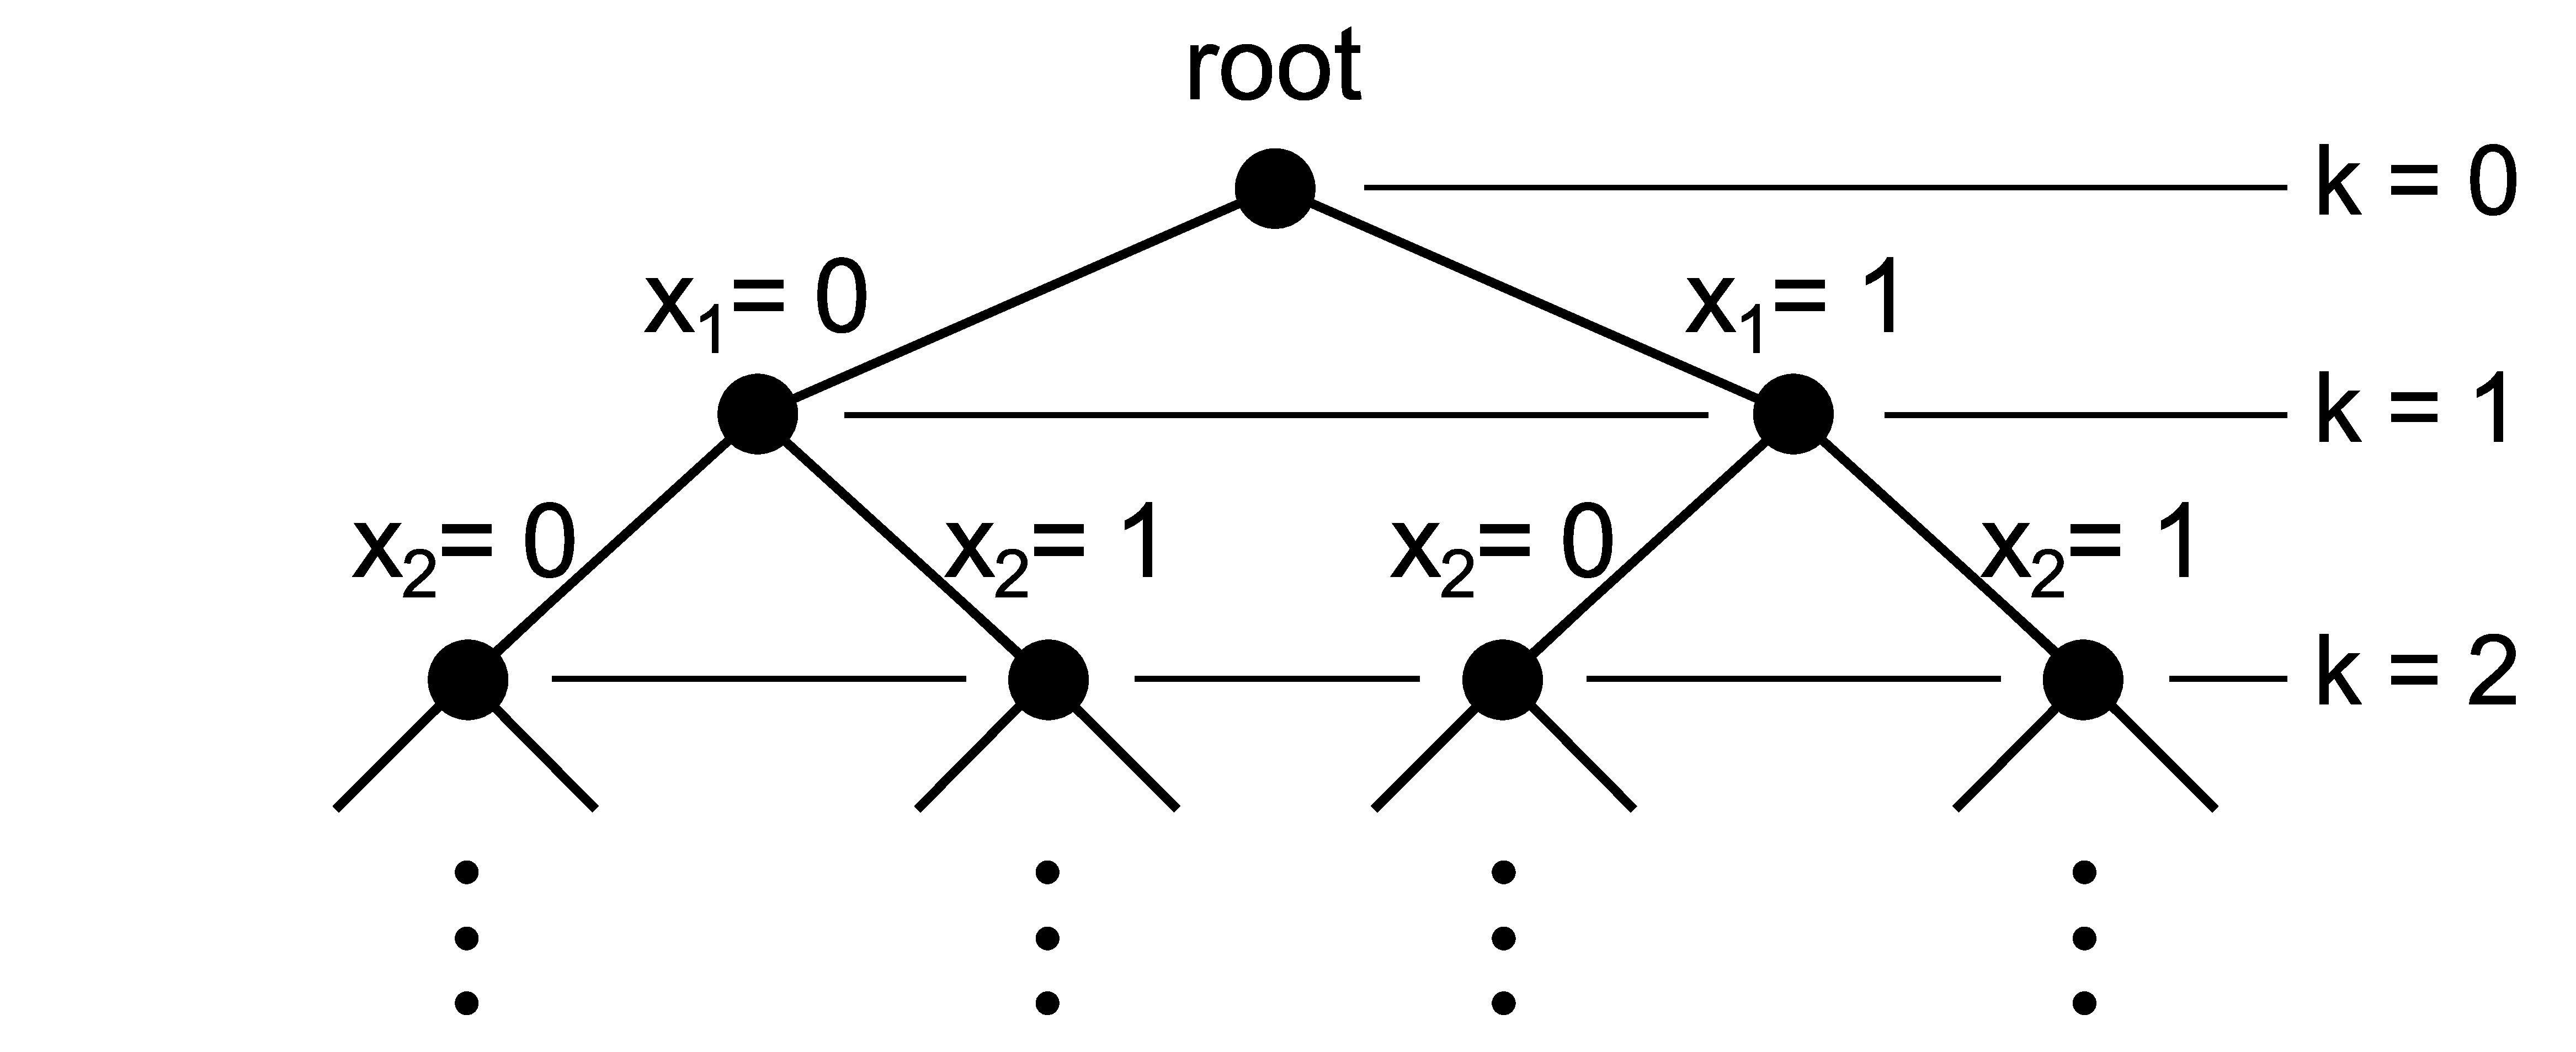
\includegraphics[width=9cm]{images/tree.pdf}
    \caption{\small{\emph{$k$-SAT representation as a search tree.}}}
    \label{fig:arvore}
  \end{center}
\end{figure}

%----------------------------------

\subsection{Observations}

At ``\emph{Dancing Links}'' \cite{knuthDLX} D. Knuth shows that choosing the column to be covered as the one with lesser elements, at each stage of the backtracking procedure, leads to a search tree with lesser amount of nodes.
This is an important observation specially for larger problems, because fewer updates (insertion and removal of elements) is realized.
For this reason it's worth to include a counter $S$ in the column structure shown above (where this counter is named as \texttt{len}).
The way the $k$-SAT problem was constructed here, the counter $S$ are only used as a criteria when covering the secondary columns, since the primary always have the same amount of elements (representing the values true and false of a literal).
Another optimization mentioned by D. Knuth is to not cover columns with no elemnts, which again does not apply to the primary columns of the $k$-SAT problem.

In addition to the structures presented previously in \texttt{Section \ref{sec:algX}}, two other data structures were created to deal with the program output, which has to be given in terms of the boolean variables (for the example shown in \texttt{Setion \ref{sec:ksatcover}}, the solution represented by the rows $x_{_1} = 1$, $x_{_2} = 1$, $x_{_3} = 1$ and $x_{_4} = 0$ should be output as 1110).
To this end, the follow structure was used to point and identify the rows of the problem:
\\[-5pt]

\linespread{0.8}

{\footnotesize
  \begin{quote}
\begin{verbatim}
typedef struct line_struct {
   node *nodeR; /* first node of a row */
   char nameR[max_name]; /* row name */
} line;
\end{verbatim}
  \end{quote}
}

\linespread{1.5}

\noindent and another structure was used to store the found solutions containing a array of the type \emph{line} above with the solutions rows, an integer indicating the search level at which the solution was found (relevant only for the exact cover problem) and a pointer to the next solution:
\\[-5pt]

\linespread{0.8}

{\footnotesize
  \begin{quote}
\begin{verbatim}
typedef struct sol_struct {
   line *rowSol; /* array of solution rows */
   int level; /* amount of rows from solution */
   struct sol_struct *next; /* pointer to the next solution */
} solution;
\end{verbatim}
  \end{quote}
}

\linespread{1.5}


%---------------------------------------------------------------------

\section{Results and Critical Point Analysis}

The probability that a $k$-CNF being satisfiable depends on the amount of clauses ($m$) and of literals ($n$).
If the amount of clauses to be satisfied is large and the mount of literals is small, then smaller is the chances of the $k$-CNF being satisfiable.
On the other hand, if the number of literals is large and the amount of clauses is small, then higher are the chances of the $k$-CNF to be satisfiable.
It is believed that for all $k$ there exists a constant $c_k$ with the following property:

\begin{quote}
  \emph{Let $\varepsilon$ a constant and suppose that $n \to \infty$.
  If $m \geq \left( c_k + \varepsilon \right) n$, then the $k$-CNF is almost-certainly not satisfiable, while if $m \leq \left( c_k - \varepsilon \right) n$, then it is almost-certainly satisfiable.}
\end{quote}

To estimate the constant $c_k$ for different values of $k$, the routine ``\emph{random\underline{ }ksat.py}'' from H. Yuen and J. Bebel has been used to generate pseudo-random instances of $k$-CNF\cite{yuen}, with a small modification to fulfill the input format described above.
For a fixed value of $k$, the quantities $n \geq k$ and $m \geq 1$ were varied and, for each triple $\left( k , \, n , \, m \right)$ a total of 50 pseudo-random instances of $k$-CNF were generated, from where the mean values of the amount of solutions and the execution time were calculated.
Such procedure can be evaluated with the following example script (for larger $n$ the size of the increment of $m$ has to be increase accordingly):

\newpage

\linespread{0.8}

{\footnotesize
\begin{verbatim}
  #!/bin/bash

  for k in `seq 2 5`
  do
    for n in `seq ${k} 20` # number of variables n: [k;20]
    do
      m=1
      aux=10 # just to get into the loop
      while [ ${aux} -gt 0 ] # while satisfiable, clauses m: [1;...]
      do
        count=0
        time=0
        for i in `seq 50` # 50 calculations, then take the mean
        do
          # Generate random input (k, n, m).
          python random_ksat.py ${k} ${n} ${m} -1 CriticalPointAnalysis/input

          ini=$(date +%s%N) # initial time

          # Execute the 'satisfyme' code.
          count=$(( ${count} + `./satifyme -n < CriticalPointAnalysis/input` ))

          fin=$(date +%s%N) # final time

          # Calculate the time in seconds.
          time=`echo "scale = 10; ${time} + (${fin} - ${ini})/1000000000" | bc`

        done

        # Calculate the mean values of the amount of solutions and the execution time.
        count=`echo "scale = 10; ${count} / ${i}" | bc`
        time=`echo "scale = 10; ${time} / ${i}" | bc`
        echo ${m} ${count} >> CriticalPointAnalysis/saida_k${k}_n${n}
        echo ${m} ${time} >> CriticalPointAnalysis/time_k${k}_n${n}

        aux=`echo "${count} / 1" | bc`
        m=$(( ${m} + 1 ))

      done
    done
  done
\end{verbatim}
}

\linespread{1.5}

The obtained estimates for the constant $c_k$ are shown in the \texttt{Table \ref{tab:result}} below:
\\[-5pt]

\begin{table}[h]
  \begin{center}
    \begin{tabular}{l c c c c c c}
      \hline
      $k$ & 2 & 3 & 4 & 5 & 8 & 10 \\
      $c_k$ & 2.44 & 5.18 & 10.76 & 21.87 & 177.00 & 709.79 \\
      \hline
    \end{tabular}
    \caption{\small{\emph{Obtained estimates for the constant $c_k$.}}}
    \label{tab:result}
  \end{center}
\end{table}

The graphs below show the mean values of the amount of solutions (log scale in both axis) and the execution time the plots (log sale in time), as a function of the number of clauses $m$ and for different number of literals $n$.
One observes that for $m \approx c_k n$, the execution time is fairly higher.

\begin{figure}[htbp]
  \begin{center}
    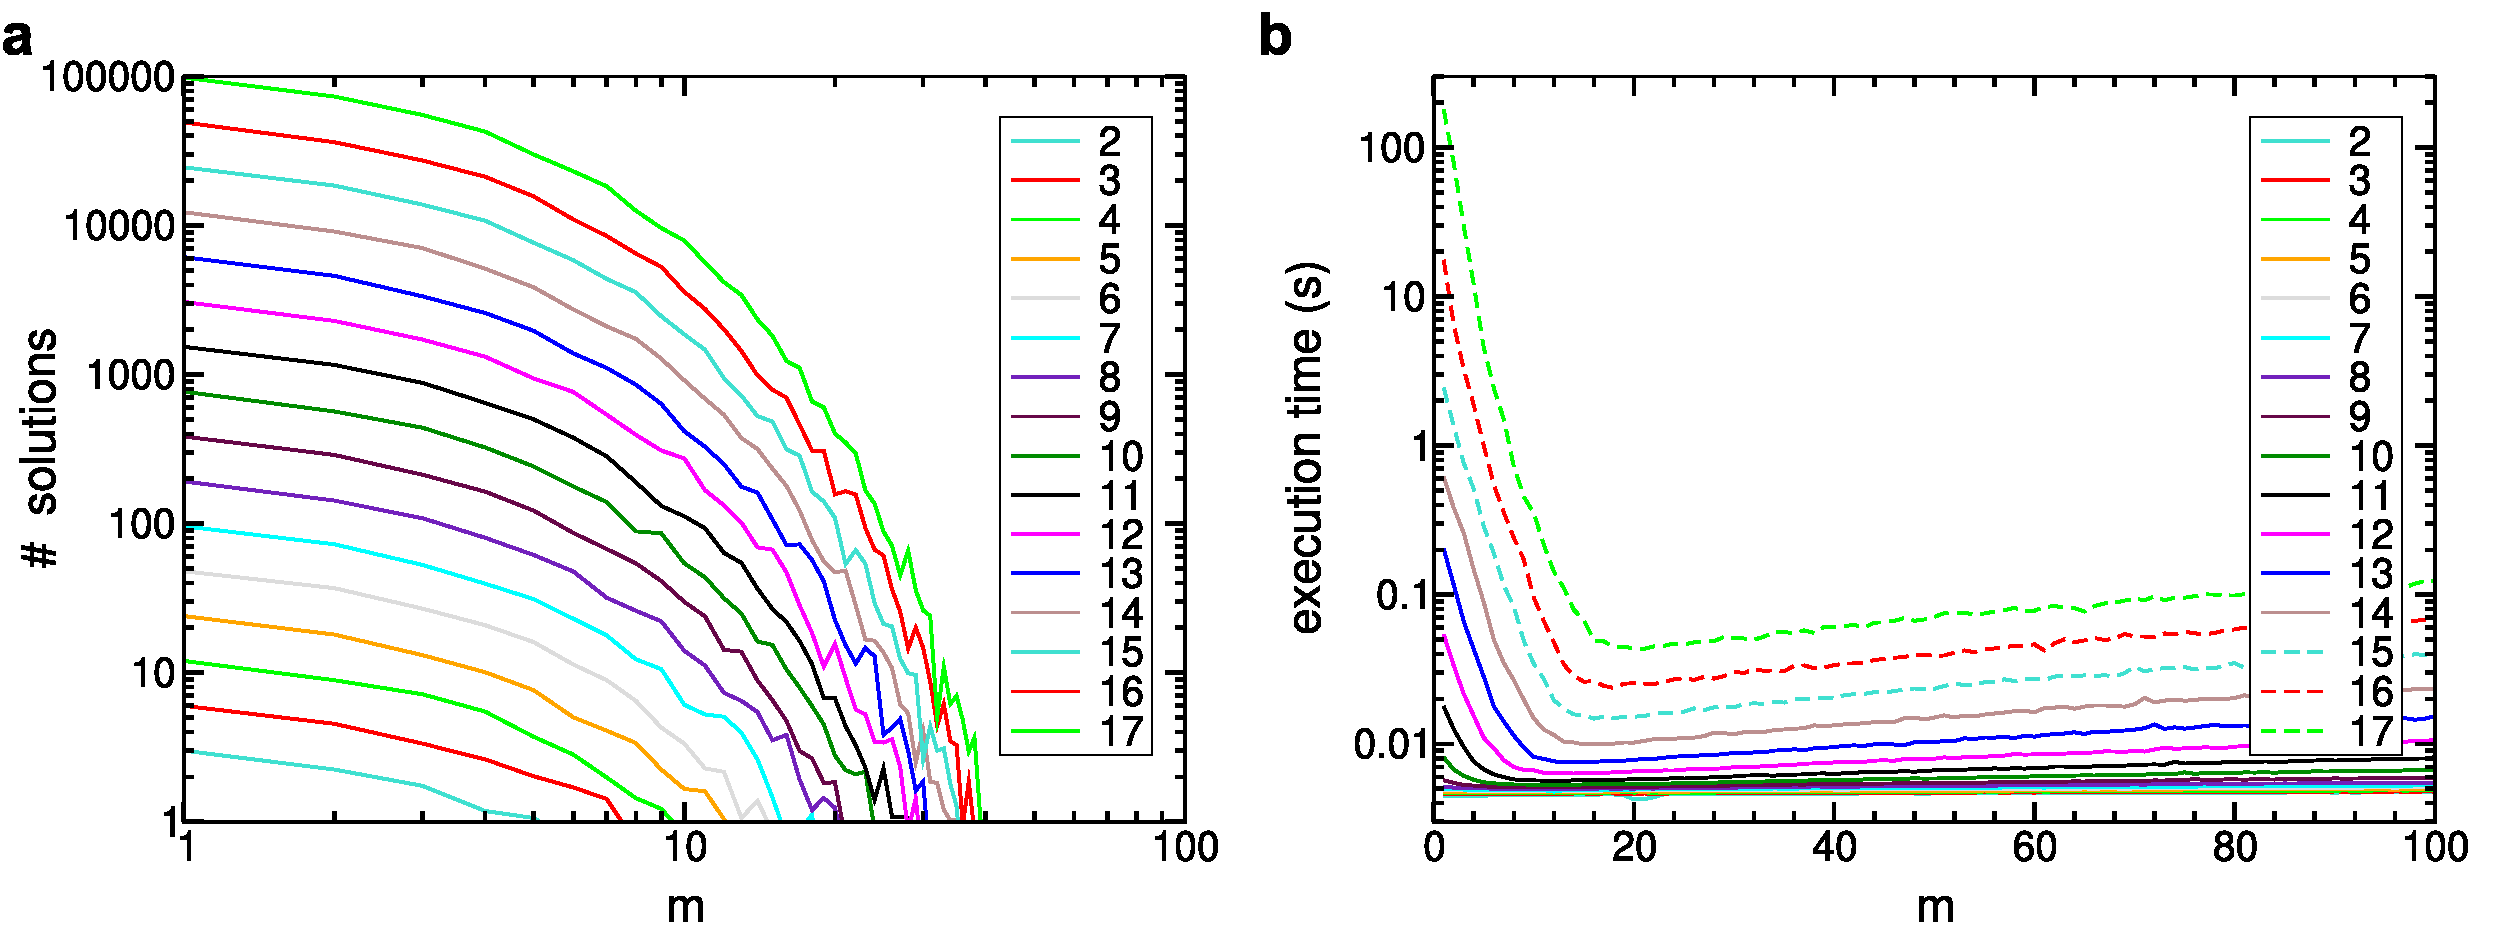
\includegraphics[width=15.2cm]{images/k2st.pdf}
    \caption{\small{Mean values of the amount of solutions ({\bf a}) and execution time in seconds ({\bf b}) of a {\bf 2}-CNF as a function of $m$ (number of clauses), taken for different $n$ (number of literals shown at the legend).}}
    \label{fig:k2}
  \end{center}
\end{figure}

\begin{figure}[htbp]
  \begin{center}
    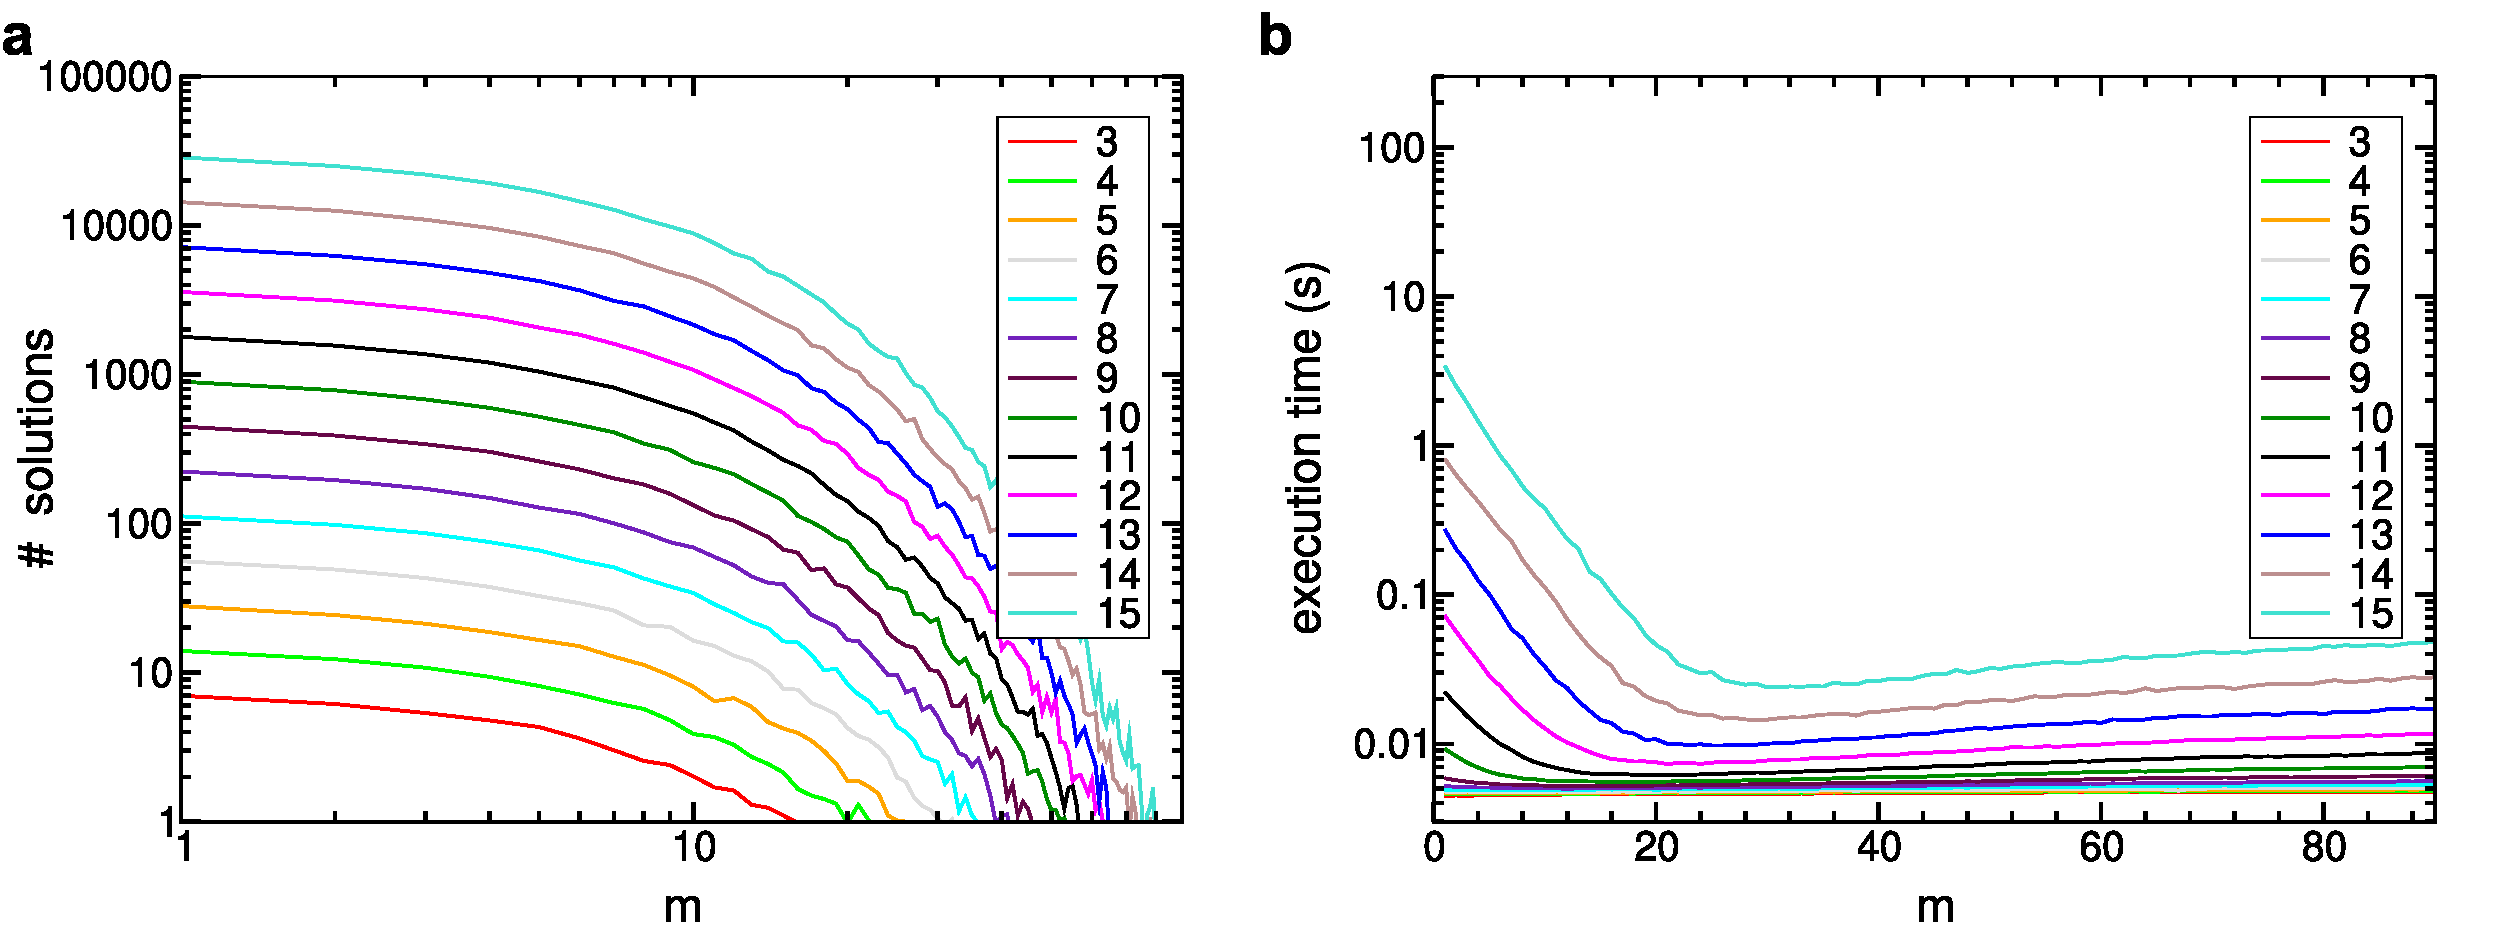
\includegraphics[width=15.2cm]{images/k3st.pdf}
    \caption{\small{Mean values of the amount of solutions ({\bf a}) and execution time in seconds ({\bf b}) of a {\bf 3}-CNF as a function of $m$ (number of clauses), taken for different $n$ (number of literals shown at the legend).}}
    \label{fig:k3}
  \end{center}
\end{figure}

\begin{figure}[htbp]
  \begin{center}
    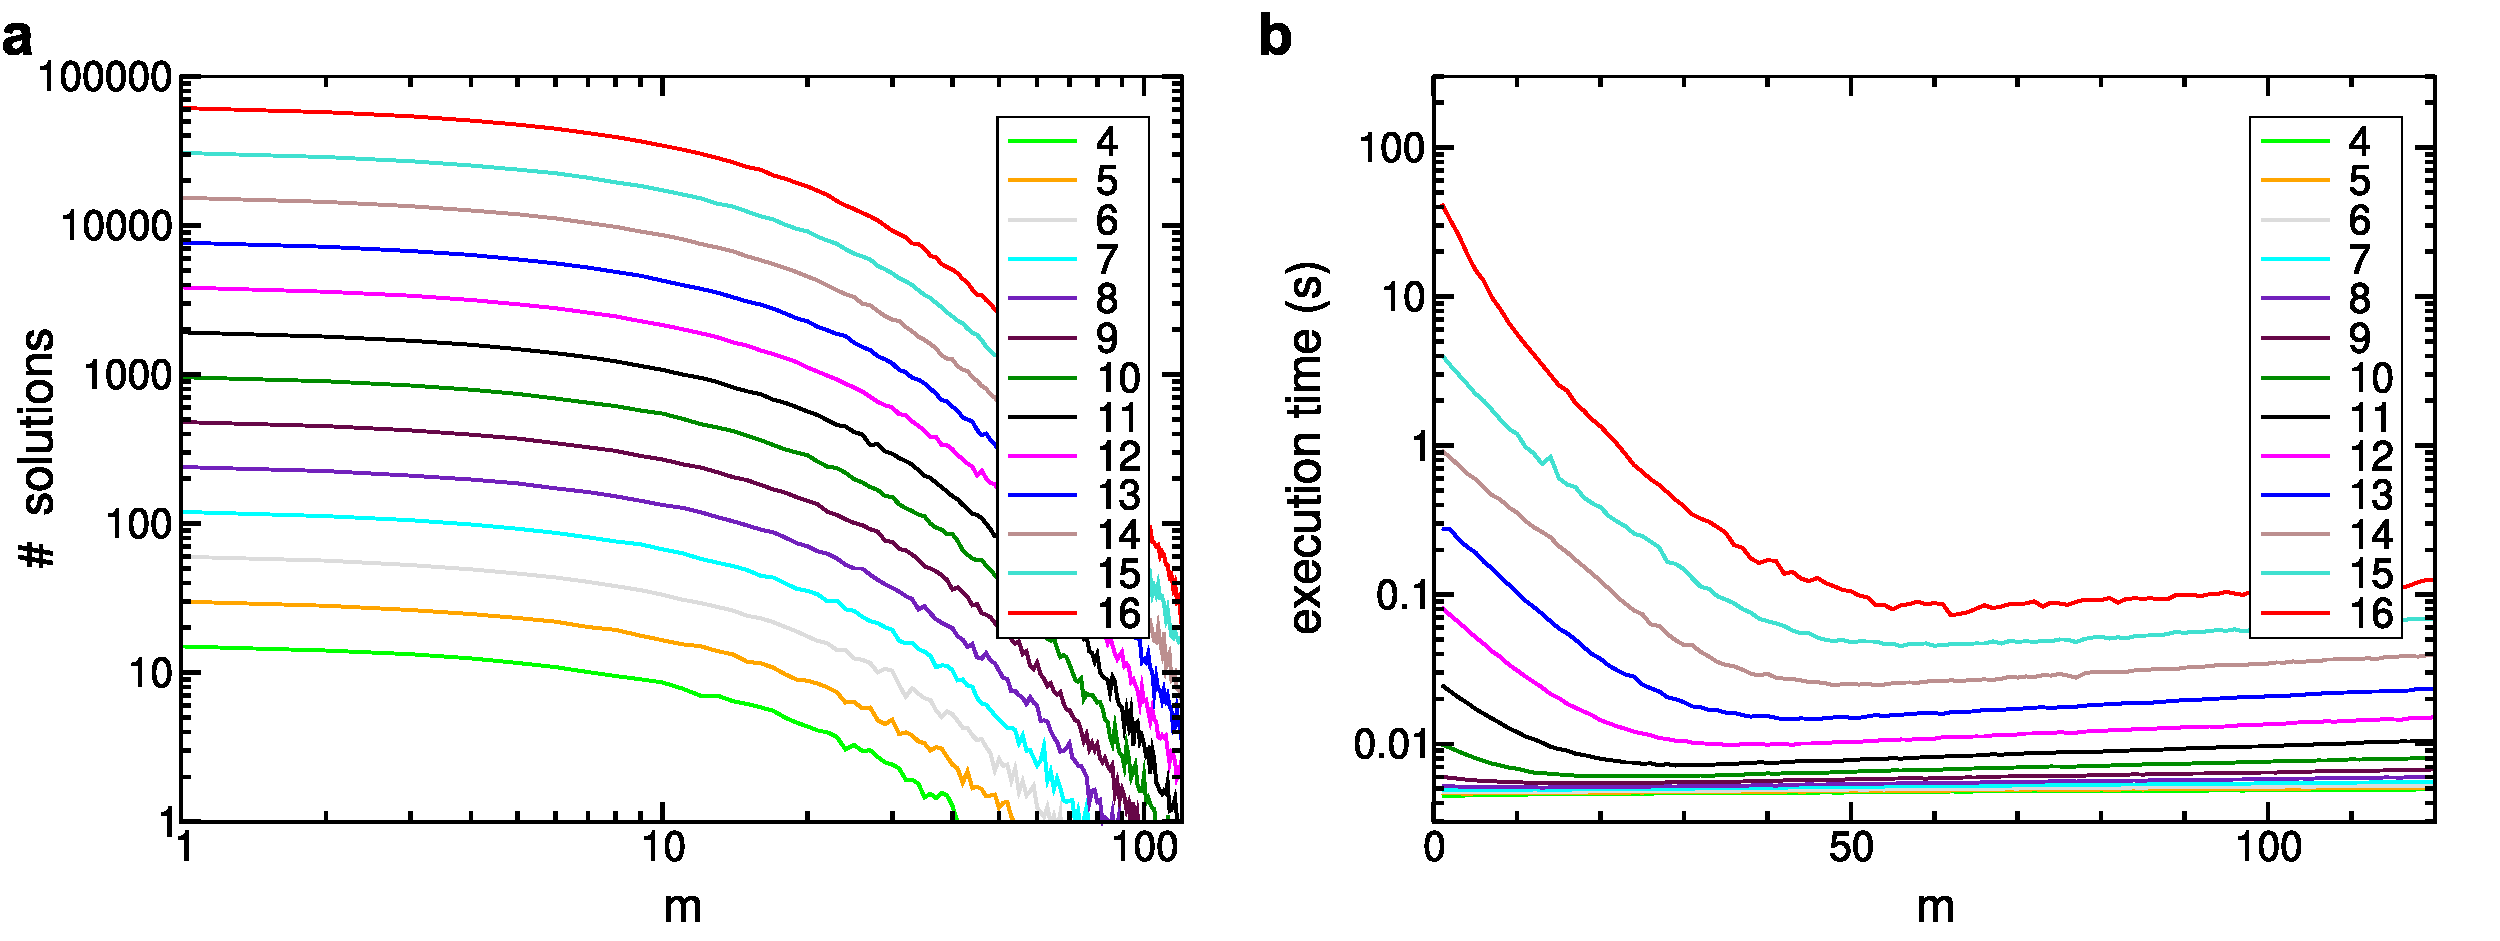
\includegraphics[width=15.2cm]{images/k4st.pdf}
    \caption{\small{Mean values of the amount of solutions ({\bf a}) and execution time in seconds ({\bf b}) of a {\bf 4}-CNF as a function of $m$ (number of clauses), taken for different $n$ (number of literals shown at the legend).}}
  \end{center}
\end{figure}

\begin{figure}[htbp]
  \begin{center}
    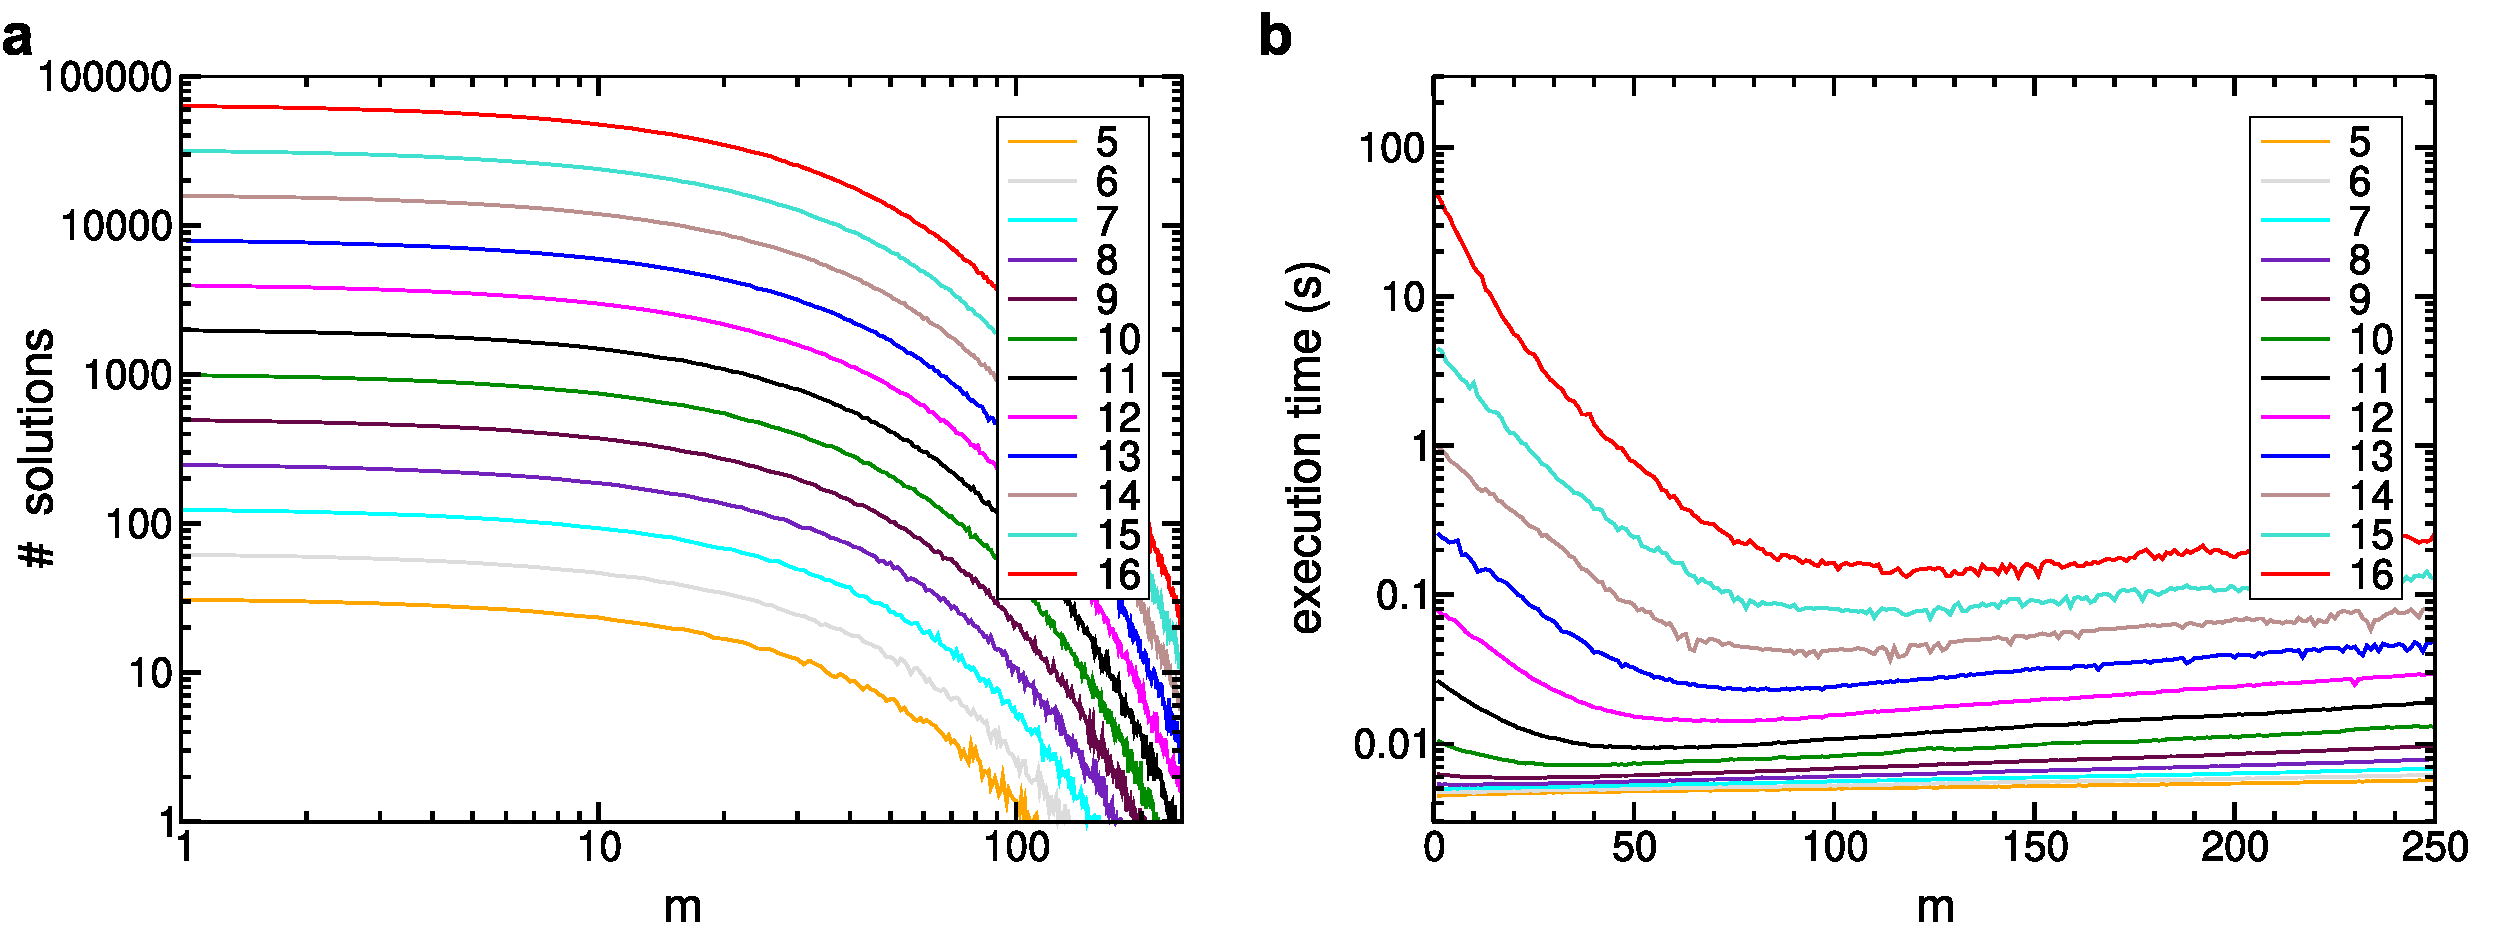
\includegraphics[width=15.2cm]{images/k5st.pdf}
    \caption{\small{Mean values of the amount of solutions ({\bf a}) and execution time in seconds ({\bf b}) of a {\bf 5}-CNF as a function of $m$ (number of clauses), taken for different $n$ (number of literals shown at the legend).}}
    \label{fig:k5}
  \end{center}
\end{figure}

\begin{figure}[htbp]
  \begin{center}
    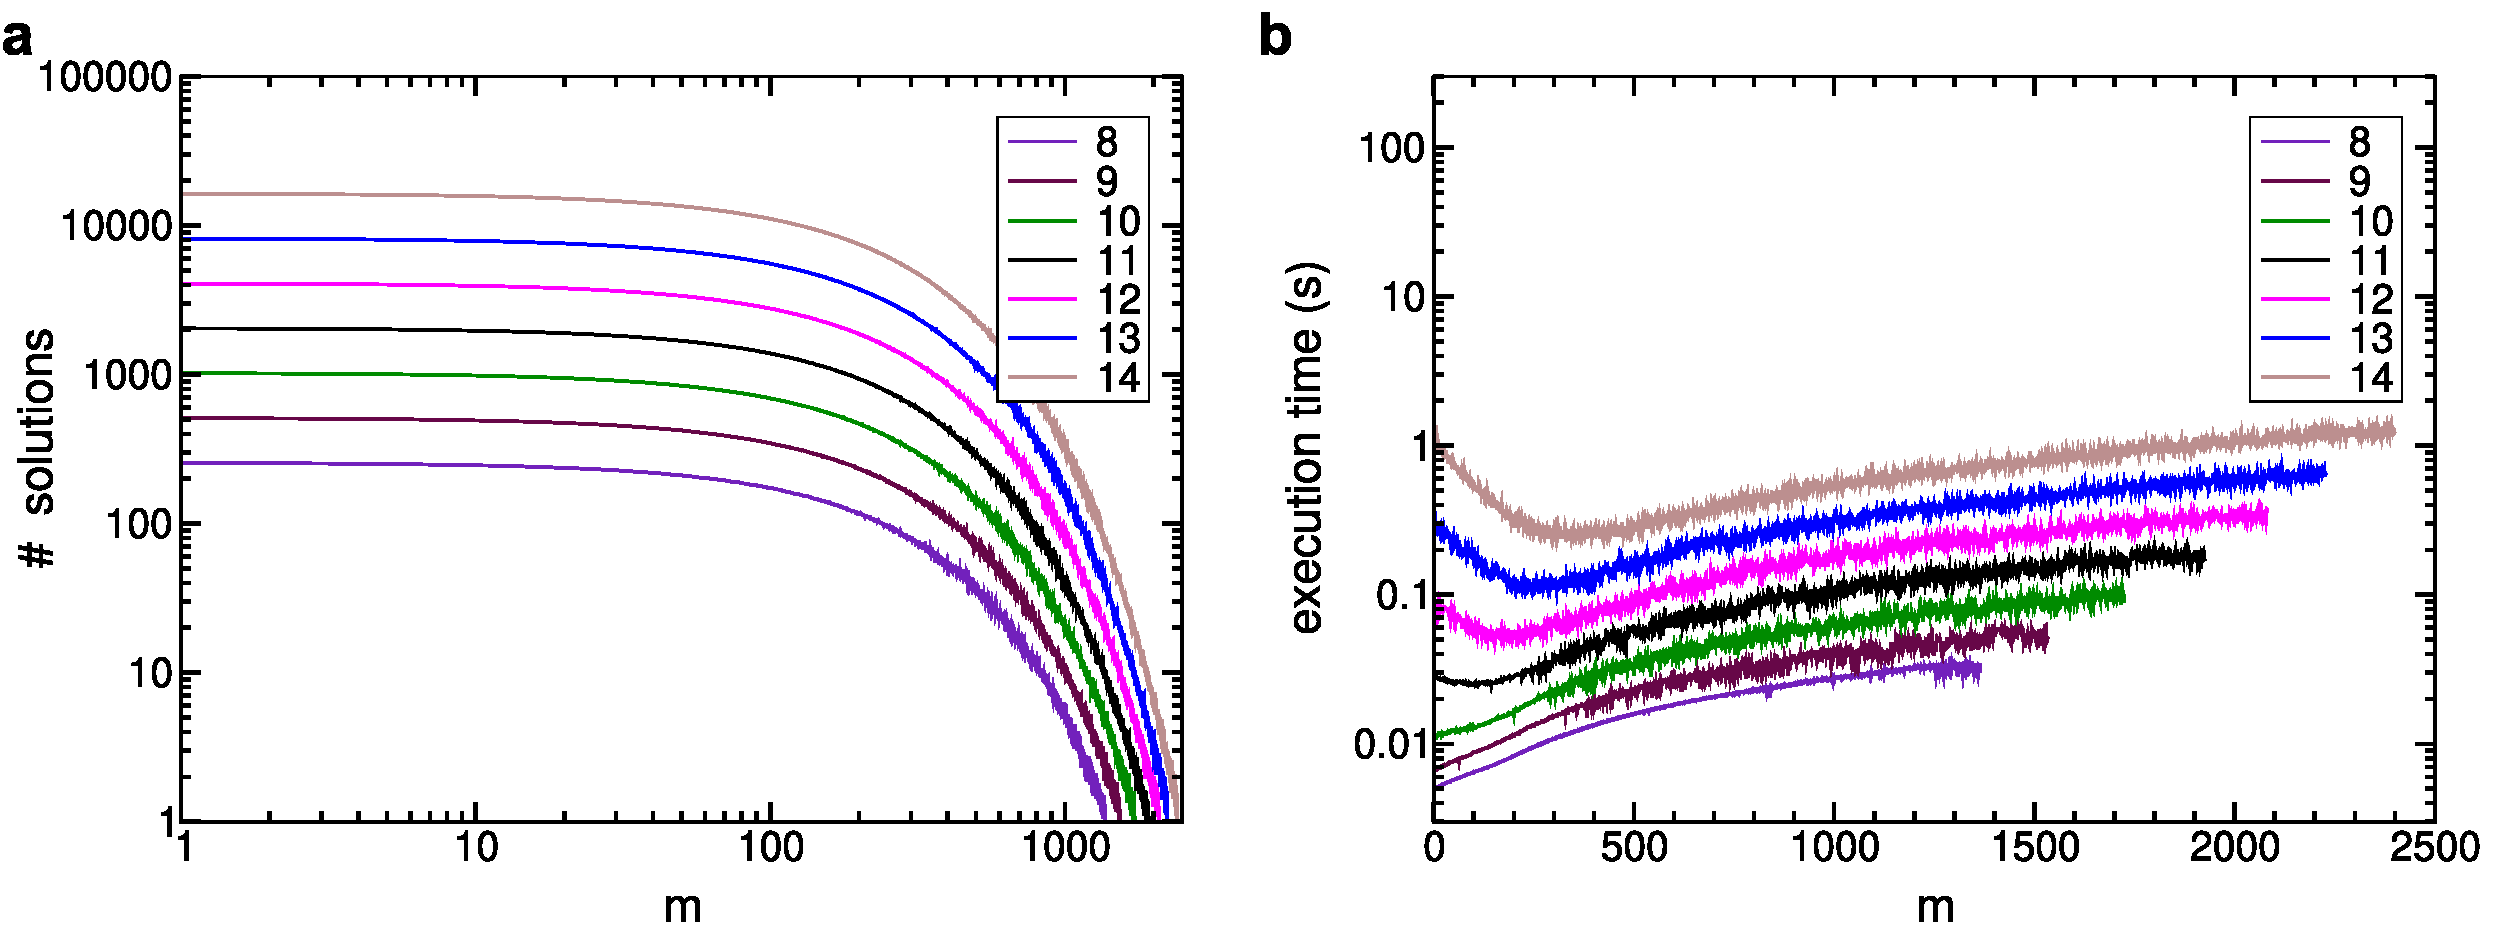
\includegraphics[width=15.2cm]{images/k8st.pdf}
    \caption{\small{Mean values of the amount of solutions ({\bf a}) and execution time in seconds ({\bf b}) of a {\bf 8}-CNF as a function of $m$ (number of clauses), taken for different $n$ (number of literals shown at the legend).}}
    \label{fig:k8}
  \end{center}
\end{figure}

\begin{figure}[htbp]
  \begin{center}
    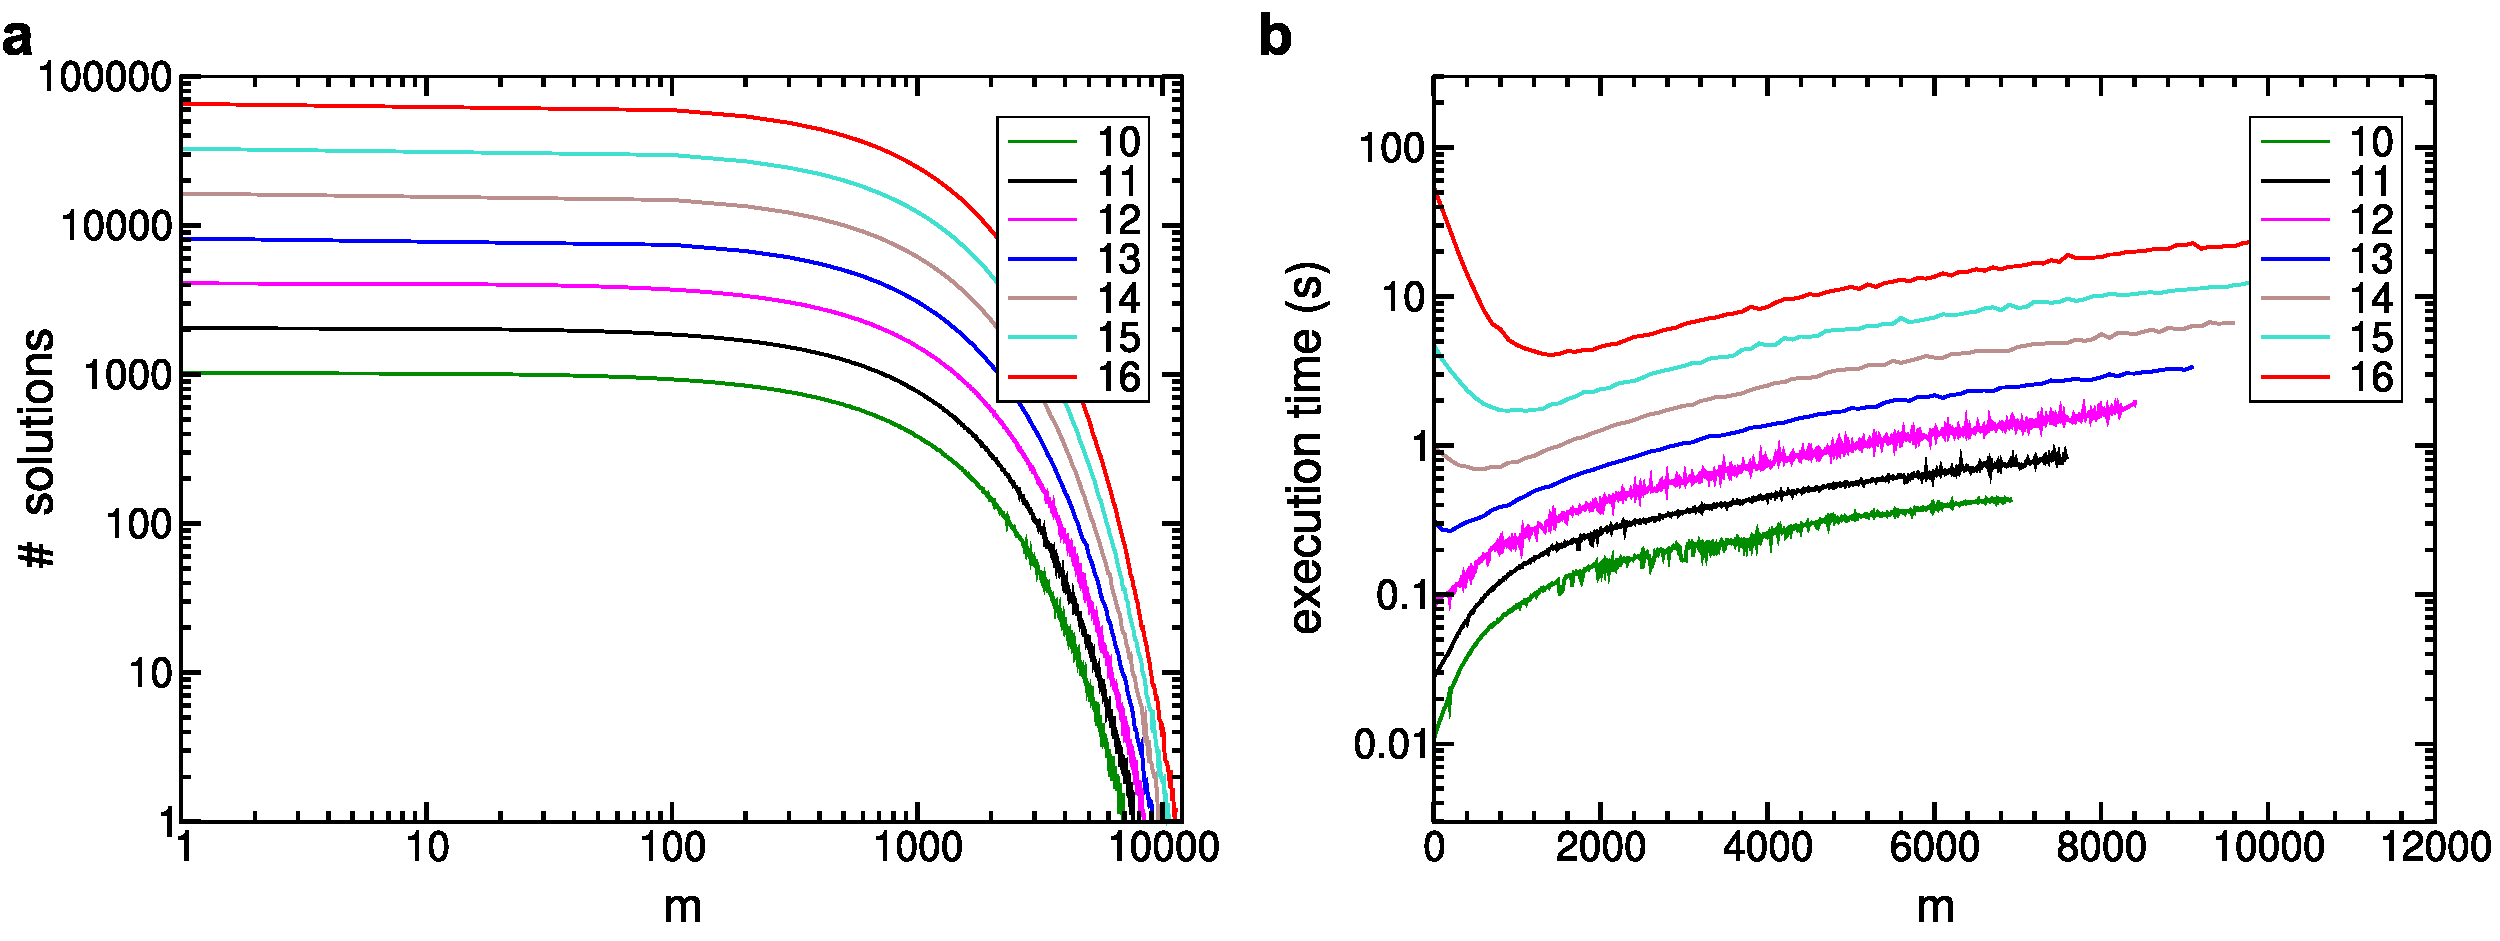
\includegraphics[width=15.2cm]{images/k10st.pdf}
    \caption{\small{Mean values of the amount of solutions ({\bf a}) and execution time in seconds ({\bf b}) of a {bf 10}-CNF as a function of $m$ (number of clauses), taken for different $n$ (number of literals shown at the legend).}}
    \label{fig:k10}
  \end{center}
\end{figure}


%---------------------------------------------------------------------

\begin{thebibliography}{2}

\bibitem{knuthDLX} D. Knuth, ``\emph{Dancing Links},'' arXiv:cs/0011047 (2000), \url{https://arxiv.org/abs/cs/0011047}.

\bibitem{yuen} H. Yuen and J. Bebel, ``\emph{ToughSat Project},'' (2011), \url{http://toughsat.appspot.com}, routine \texttt{random\underline{ }ksat.py} consulted in April 20$^\text{th}$, 2012.

\end{thebibliography}

\end{document}


